\chapter{Grid generation}\label{cha:grid-gen}
In this chapter we discuss methods that allows us to apply our prior knowledge directly into the grid generation process.
This is a stark contrast to the methods in the previous chapter which helped us
to impose our constraints in the learning process.
Even though these methods worked despite limited prior knowledge, they have
one major drawback:
We \emph{always} have to generate a complete sparse grid.
This was not a problem for the lower dimensional datasets we used to evaluate
the methods, but is a limiting factor for higher dimensional problems.
\sidetitle{High dimensional problems}
To tackle very-high dimensional problems, we need to be able to influence the
grid generation.

The first method discussed here, generalized sparse grids, allows us to impose
further smoothness constraints on the grid.
The second method, interaction-term aware sparse grids, allows us to impose
knowledge about the possible variable interactions on the grid.

\section{Generalized Sparse Grids}\label{sec:generalised-sg}
Generalised sparse grids are a technique that allows us to influence the
granularity of the grid.
They were first developed by \citeauthor{optimizedApproxSpaces} in~\cite{optimizedApproxSpaces}.

\subsection{Theory}
%Maybe use index set notation?
Despite the fact that the generalised sparse grid techniques originates from
complicated calculations, they are stated by two simple formulas.
We only need to change \vref{eq:sparse-grid-space} to generalise our grid.
We can describe the set of grid points for the generalised sparse grid \(G^T_n\)
of level \(n\) and its corresponding approximation space \(V^T_n\) with
\begin{align}\label{eq:generalised-grid-space}
G_n^T &= \bigcup_{\mathclap{\substack{\vert {\bm{l}} \vert_1 - T \vert \bm{i} \vert_\infty \\ \leq n + d - 1 - T n}}} G_{\bm{l}},\\
V_n^T &= \bigoplus_{\mathclap{\substack{\vert {\bm{l}} \vert_1 - T \vert \bm{i} \vert_\infty \\ \leq n + d - 1 - T n}}} W_{\bm{l}}.\nonumber
\end{align}
The constant \(T\) can be chosen in the interval \((-\infty, 1]\) and governs
our choice of subgrids.
Setting \(T\) to zero recovers the standard sparse grid, higher values
approaching one transform the grid to the form seen in figure x.
The limit \(T \to -\infty\) corresponds to a full grid.
Note that, even if the value of \(T\) is continuous, it acts as a discrete
operator.
The actual value of \(T\) does not matter, different values can result in the
same grid.
The dimension of the generalised sparse grids with level \(n\) and constant
\(T\) can be described by
\begin{equation*}
  \operatorname{dim}(V^T_n) \leq
  \begin{cases}
    d 2^n & T = 1, \\
    \BigO(2^n) & T \in (1/n, 1),\\
    \BigO(2^n n^{d-1}) & T \in [0, 1/n],\\
    \BigO(2^{\frac{T - 1}{T/d - 1} n}) & T < 0.
  \end{cases}
\end{equation*}
We can see that the special cases \(T = 0\) and \(T \to \infty\) are covered~\cite{optimizedApproxSpaces}.
\todo{Write about interpolation error and check dimensionality formula.}

A higher value of \(T\) decreases the amount of grid points and interaction terms.
The effect for a grid with dimension 4 and level 5 can be seen in \cref{fig:adaptivity}.
\begin{figure}[thb]
\makebox[\textwidth][c]{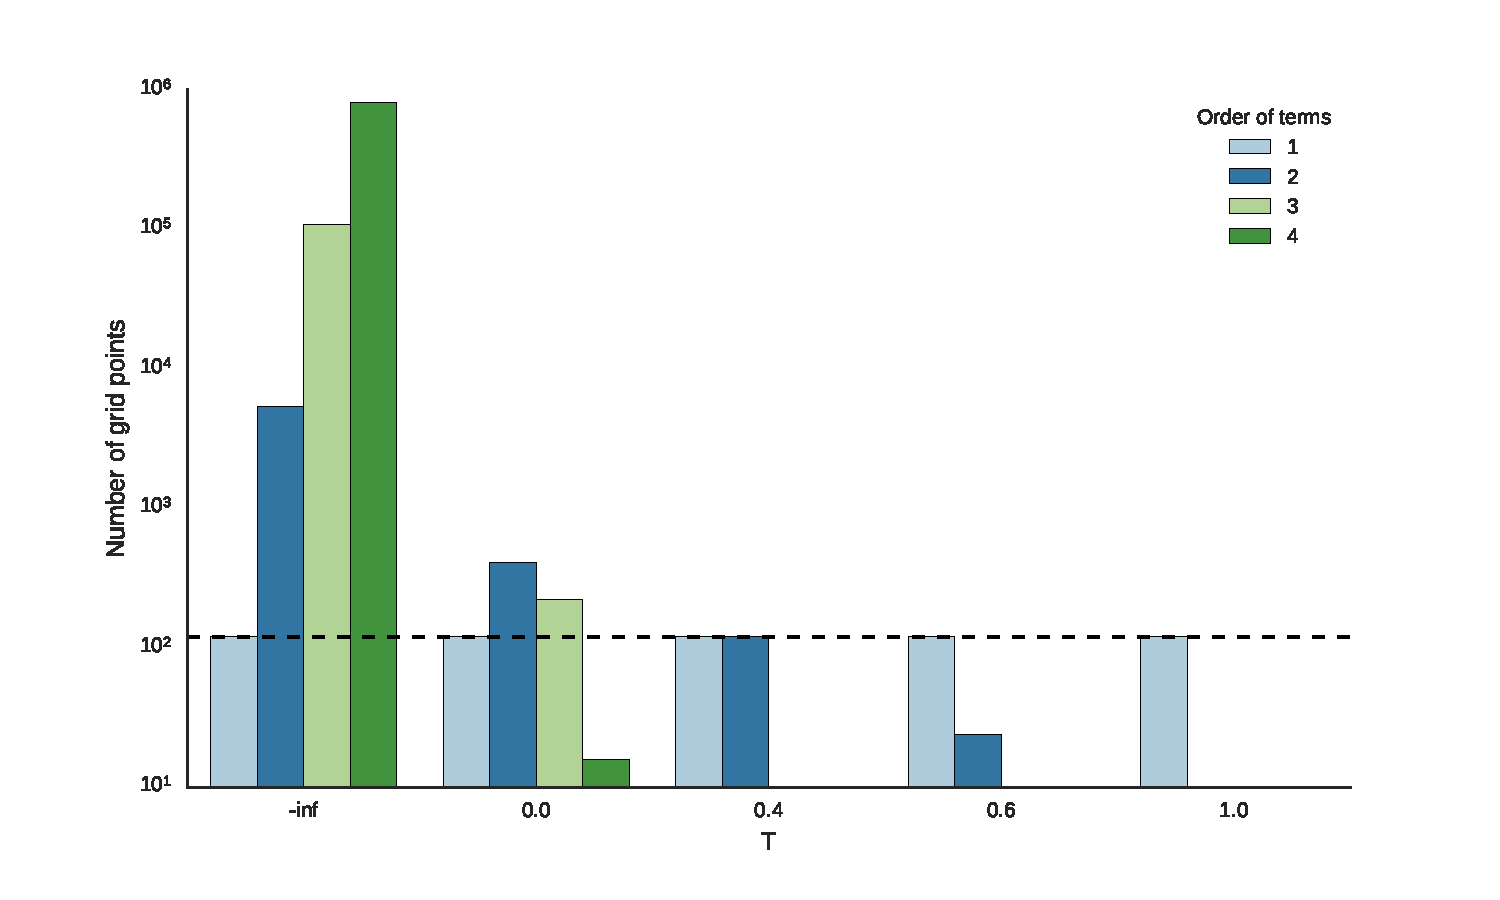
\includegraphics[width=1.2\textwidth]{interactionT}}%
\caption[Order of interaction terms for generalised sparse grids.]{
This figure shows the number of terms of each order for a grid with dimension 4
and level 5.
The bias term is not included in the graphic, it is contained in all grids.}\label{fig:adaptivity}
\end{figure}
Note that the grid for \(T = 1\) does not contain any interaction terms.
The number of grid points of order one, i.e.~points that are constant for all
but one variable stay the same.
The grid for \(T = 1\) does not contain any points except the aforementioned
ones.

\begin{figure}[H]
  \centering
  \begin{subfigure}[b]{0.23\textwidth}
    \centering
    \includegraphics[width=\textwidth]{{{grid_T-inf}}}
    \caption{\(T = -\infty\)}
  \end{subfigure}
   \begin{subfigure}[b]{0.23\textwidth}
    \centering
    \includegraphics[width=\textwidth]{{{grid_T0}}}
    \caption{\(T = 0.0\)}
  \end{subfigure}
 \begin{subfigure}[b]{0.23\textwidth}
    \centering
    \includegraphics[width=\textwidth]{{{grid_T0.5}}}
    \caption{\(T = 0.5\)}
  \end{subfigure}
 \begin{subfigure}[b]{0.23\textwidth}
    \centering
    \includegraphics[width=\textwidth]{{{grid_T1.0}}}
    \caption{\(T = 1.0\)}
  \end{subfigure}
  \caption{Grid visualization for different \(T\)s}\label{fig:grids-T}
\end{figure}

\subsection{Implementation}
The implementation is quite simple, at least in our case.
It was possible to change the already existing grid generation algorithm.
The changes amounted to simply modifying the inclusion criterion so that it
reflect the criterion described by \cref{eq:generalised-grid-space}.

\begin{algorithm}[h]
 \caption{Generalised Sparse Grid Generation}\label{alg:gen-sg} 
 \begin{algorithmic}[1]
   \Require{???}
   \Statex
   \Function{GridGeneration}{params}
   \For{\(0 \leq d \leq \text{ dimensions}\)}
   \State\Call{CreatePoint}{0, 1, 1} \Comment{Bias points}
   \EndFor
   \For{\((l, i) \in \{ 1 \leq l \leq n, 1 \leq i < l^2, i \text{ odd} \} \)}
     \State\Call{CreatePoint}{0, l, i} \Comment{1d-grid points for first dimension}
   \EndFor
   \For{\( d \in \text{dimensions}\)}
   \For{\(p \in \Call{GetAllGridPoints}{}\)}
   \Let{levelSum}{\Call{p.getLevelSum}{} - 1}
   \Let{levelMax}{\Call{p.getLevelMax}{}}
   \Let{l}{1}
   \While{\(\max(l, \text{levelMax}) \leq n\)}
   \Let{left}{\((l + \text{ levelSum}) - (T \cdot \max(l, \text{ levelMax}) \)}
   \Let{right}{\((n + \text{ dimensions} - 1) - (T \cdot n)\)}
   \If{left \(>\) right}
   \State\Call{break}{}
   \EndIf
   \For{\(1 \leq i < 2^l, i \text{ odd}\)}
   \State\Call{CreatePointAt}{d, l, i, p}
   \EndFor
   \Let{l}{l + 1}
   \EndWhile
   
   \EndFor
   \EndFor
   \EndFunction
 \end{algorithmic}
\end{algorithm}

\subsection{Results \textit{\&} Discussion}
\newenvironment{ttable}{
  \begin{tabular}[c]{S[table-format=2.1]
    S[table-format=1.4, table-figures-exponent=2, table-sign-mantissa, table-sign-exponent]
    S[table-format=4.1(4)]
    S[table-format=2.1]
    c
    c
    S[table-format=2.3]
    S[table-format=2.3]}
  \toprule \multicolumn{1}{c}{\(T\)}
& \multicolumn{1}{c}{\(\lambda\)}
& \multicolumn{1}{c}{\textsc{cv}-Grid}
& \multicolumn{1}{c}{\textsc{cv-rmse}}
& \multicolumn{1}{c}{Train-Grid}
& \multicolumn{1}{c}{Train-\textsc{rmse}}
& \multicolumn{1}{r}{Test-\textsc{rmse}}
\\\midrule}{\bottomrule\end{tabular}}

Generalised grids work well in theory.
To test their practical performance, we tested two things that we will discuss
in this section:
\begin{enumerate}
\item In what way does the grid parameter \(T\) influence the regularization
  parameter \(\lambda\)?
\item Can we archive a better performance with generalised sparse grids compared
  to standard grids, with a comparable number of grid points?
\end{enumerate}
\todo{Train-Grid should be an integer!}
\begin{table}[tb]
    \begin{ttable}
-0.5 & 2.2762e-10 & 5541.3( 185) & 1.246 & 5547.0 & 0.823 & 1.226\\
0 & 1.4539e-04 & 2278.8(  33) & 1.196 & 2277.0 & 0.845 & 1.179\\
0.5 & 7.7081e-05 & 640.8( 141) & 1.051 & 651.0 & 0.959 & 1.028\\
1 & 1.0432e-04 & 391.2(  72) & 1.031 & 395.0 & 0.976 & 1.015\\
    \end{ttable}
\caption[T vs \(\lambda\) for friedman1 dataset.]{Best results and used \(\lambda\) for different
  \(T\)s for the Friedman1 dataset and an estimator with level 4}\label{fig:t-vs-mse-friedman1}
\end{table}

\begin{table}[b]
    \begin{ttable}
-0.4 & 1.9276e-02 & 8468.7( 206) & 4.703 & 8470.0 & 2.275 & 4.215\\
0 & 1.9622e-02 & 6678.3( 271) & 4.709 & 6650.0 & 2.286 & 4.184\\
0.5 & 6.2935e-03 & 1140.4( 239) & 4.771 & 1180.0 & 2.664 & 3.797\\
0.6 & 1.2700e-02 & 712.7( 242) & 4.781 & 685.0 & 3.398 & 4.308\\
    \end{ttable}
\caption[T vs \(\lambda\) for concrete dataset.]{Best results and used \(\lambda\) for different
  \(T\)s for the concrete dataset and an estimator with level 5. The optimal
  \textsc{rmse} is 1.0.}\label{fig:t-vs-mse-concrete}
\end{table}


We performed 25 iterations of a Bayesian hyper-parameter search for \(\lambda\) for the Friedman1 dataset (see \cref{sec:friedman,eq:friedman1}) with identity regularization and a generalized sparse grid for different \(T\)s and level 4.
Each learner performed five adaptivity steps refining three points each.
The results can be seen in \cref{fig:t-vs-mse-friedman1}.
In this case, the best results were archived for \(T = 1\) and the smallest grid
size, all other parameters overfit the data.
This happens, because we used a small version of the Friedman1 dataset --- it
being an artificially created dataset it would be easy, to create more samples
and then fit an arbitrarily large model.
We can see from this example, that generalised sparse grids allow us to use a
higher level, which corresponds to a larger amount of grid points with order
one, than with standard sparse grids.
Additionally the combination with adaptivity allowed us to start with an
estimator that only models few interaction terms and then creating needed
interaction points on demand.
The parameter \(\lambda\) describes the amount of regularization per
grid point.
We can see no trend in the results for the Friedman1 dataset for \(\lambda\).
A possible reason for that might be the same reason the sparse grid with \(T =
1\) showed the best result:
Except for the \(x_1 \times x_2\) interactions, the Friedman1 model has no
qualitative interactions, i.e.~they are inherently additive in effect.
This implies that the additional interaction points for larger grids would
have a rather low surplus, even for an estimator fit without regularization.
The higher-order grid points thus need a smaller amount of regularization than
the first-order terms, which explains the small \(\lambda\) for the largest
grid.
All other regularization parameters have values that are of similar order, the
differences could be caused by multiple factors.

The Friedman1 results demonstrated, that generalised grids can help us to use
grids with a level, that would lead to severe overfitting for normal sparse
grids.
We used a similar experiment for the concrete dataset, this time performing 45
Bayesian search iterations and using estimators with level five.
For this dataset the chosen level did not lead to overfitting even for the
highest value of \(T\) and we can therefore use it to discuss the trade-off
between approximation accuracy and degrees of freedom our proposed method makes.
The results can be seen in \cref{fig:t-vs-mse-concrete}.


Note that there is a correlation between grid size and the errors: larger grids
perform better, at least for the cross validation and training error metrics.
A further increase of the dimension of the approximation space would probably
soon lead to overfitting.
Even for our chosen level, we have in the \(T \geq 0.5\) cases more grid points
than training examples, which leads to an underdetermined linear system.
We can also see that the decrease in error between the largest grid and the standard sparse grid is rather small, considering the amount of additional grid points needed.
Note that the estimator with \(T = 0\) has a higher \textsc{cv}- and
train-\textsc{rmse} than the learner with \(T = -0.4\), but a lower testing
error.
This and the fact that the differences are small makes the results hard to
interpret.
We can see that the trade-off between error and discretization cost, which the generalised sparse grids make, works.
\todo{Actually make the comparison here\ldots}
If we compare the performance of the generalised sparse grid with level five and
\(T = 0.5\) with the standard sparse grid of level four, we can see that the
generalised grid performs better than the standard grid, even though they both
use a similar number of grid points.
The standard grid with level four needed xxx gridpoints for a \textsc{cv-rmse}
of xxx, which means that it performed worse for a similar number of degrees of freedom.

As an additional result, generalized sparse grids combined with the diagonal
matrix regularization functional show further potential.
An example for this can be seen in \cref{fig:tikhonov-concrete-l5}, which depicts a grid search
similar to the one in section diagonalxxx, only using level five instead of
level four and using the generalised sparse grids method with \(T = 0.5\).
, archiving \ldots.

We can conclude that our proposed method can improve the performance without
additional cost.
Because the smoothness constraints for the generalised grids are stronger than
the assumptions of the standard grid this result does not have to hold for all datasets.
Even though their performance depends on the feature interactions, it is hard to
tell the nature of them apart before actually training a model.
Therefore it seems useful and necessary, to build multiple models with different
grid types and thus include the granularity of the grid into the model selection process.

\begin{figure}[htb]
  \centering
  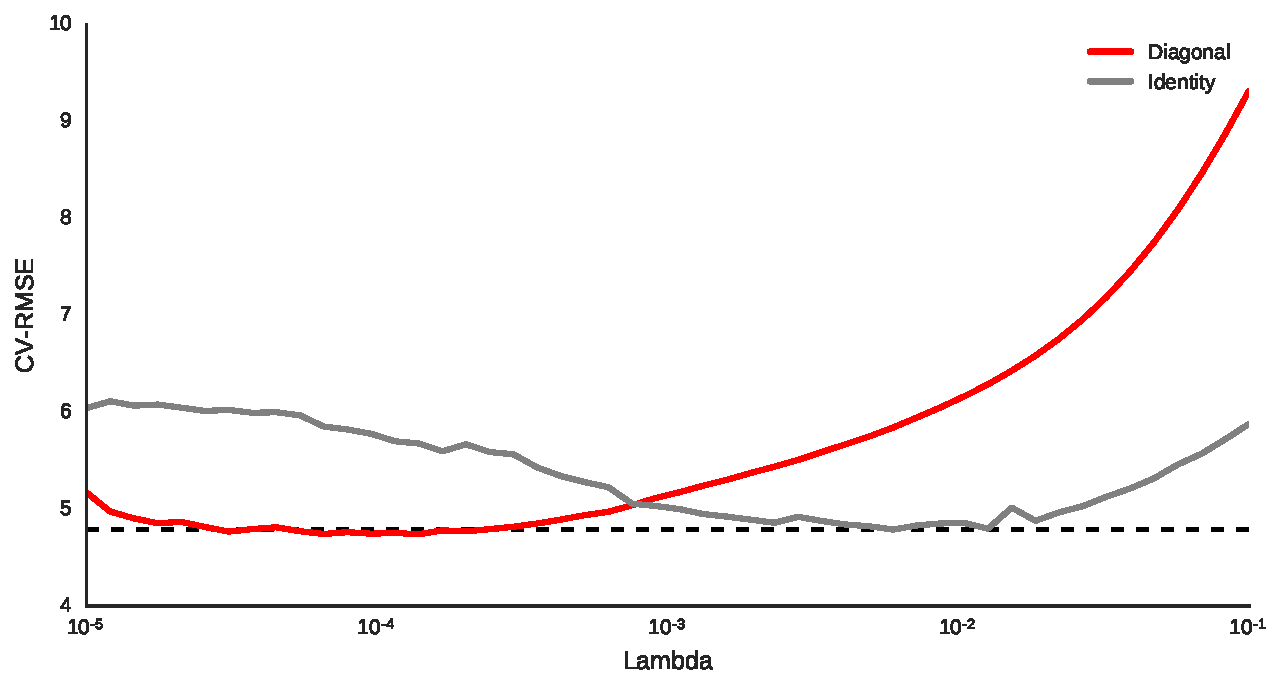
\includegraphics[width=\textwidth]{tikhonov_concrete_l5}
  \caption{This figure presents the obtained results for the concrete dataset
    obtained with estimators with level five and \(T = 0.5\).}
  \label{fig:tikhonov-concrete-l5}
\end{figure}

\section{Interaction-Term Aware Sparse Grids}
As previously noted, sparse grids not only include grid points, which model an original feature, but
also interaction points.
We discussed the usage of sparse regularization methods to select the relevant
grid points, even using a grouping of weights.

It is possible to guess the relevant interaction terms for some datasets.
For example, if we have features that represent pixels of an image, we can
exclude the interactions of pixels that are far away from each other.
Close-by pixels share more information and their interaction with each other can
reveal structure in the image, that would stay hidden without them.
Pixels that are on the opposite side probably do not share enough information to
make their inclusion worthwhile.

Consider for example an 64-dimensional dataset, where each dimension corresponds
to a pixel.
We can calculate the number of included terms for a \(d\)-dimensional dataset
discretized using a sparse grid of level \(l\) using simple combinatorics:
\begin{equation*}
  \operatorname{count-terms}(d, l) = \sum_{k  = 0}^{\max (d, l-1)} \binom{d}{k} 
\end{equation*}
If we evaluate that equation for the aforementioned 64-dimensional dataset for a
grid with level 3, we get 2081 terms.
For a grid with level 4 the same calculation results in 43745 variables.
A grid that includes such a large number of terms becomes unmanageable soon.

Let \(d\) be a metric that measures closeness between two pixels.
We can then iterate over each pixel and calculate the distance between it and
every other pixel.
If the metric is below a certain threshold, we integrate the interaction into our
model.
Note that although this is an \(\BigO(n^2)\) algorithm, it is fast enough for
our small problem instance.
Because we still deal with a low amount of pixels, in our case 64, we only need
to check 256 pairs, which is negligible compared to the actual learning
process.
We define two metrics:
\begin{align*}
  d(x_1, x_2)_{\Vert \cdot \Vert_2} &= \sqrt{(x_1 - x_2)^2 + (y_1 - y_2)^2},\\
  d(x_1, x_2)_{\Vert \cdot \Vert_1} &= \vert x_1 - x_2 \vert + \vert y_1 - y_2 \vert,
\end{align*}
which are called the Manhattan and the Euclidean distance respectively.

\subsection{Implementation}
Similar to the implementation of the generalised sparse grids we only needed to
make some small changes to the grid generation algorithm.
The idea is to pass an additional parameter to the generating function that
determines the interaction terms we want to integrate into the model.
This parameter is a list of interactions, each interaction is modelled as a list
of dimensions that should interact with each other.
The list is then converted to a hash set, that stores one boolean vector for
each interaction.
Each entry of this vector is true if the dimension should be used and false
otherwise.
We then encode each point that would be included by the standard grid generation
process in the same manner, and check if the resulting vector is included in our
hash set before it is included in the model.
This implementation strategy is efficient due to the underlying implementations.
It costs us \(\BigO(1)\) operations to check if an element is contained in the
set, which is both asymptotically optimal and efficient in practice.
The boolean vector in the \emph{C++} standard library is implemented as a bitfield, which allows us to save space.
Our proposed implementation strategy has one major drawback:
For example, if we decide to include the interaction \(x_1 \times x_2 \times
x_3\) into our model, the grid points for the pairwise interactions (e.g.~ \(x_1
\times x_2\)) are also created.
This is not a problem for statistical inference, because it is standard practice
to include all lower-order interactions anyway.
The reason for that is, that when we assume there is an interesting interaction
between multiple grid points, we also assume that the original grid points and
their interactions are relevant for the model.

\subsection{Results \textit{\&} Discussion}
We use a version of the classical \textsc{mnist}-dataset, obtained from the
\textsc{uci} machine learning repository~\cite{datasets-uci}.
The goal of this dataset is to use hand drawn pictures of one digit each to
classify the digit depicted.
Our version of the dataset is composed of 64-features, each one represents one
gray pixel, all features are in the range 0--15.
Trying to construct a sparse grid for such a highly dimensional dataset is
possible for small levels and becomes highly intractable for larger levels.
This is why we need to exclude most of the interaction terms.
We used algorithm xxx to select the neighbors for each pixel, and only include
the nearest neighbors in our grid.
This was done using the Euclidean distance with a threshold of \(\sqrt{2}\),
which leads to a \(3 \times 3\) convolution.
An example of this can be seen in figure xx.
The effect on the grid sizes for some different metrics are shown in table xxx.

Because we have to train one regression learner for each class it takes a rather
long time to generate a model, which in practice means that a grid search for
the regularization parameter was infeasible.
This is why we tried to find an approximation by using only a three-class subset
of the dataset for this purpose.
The smaller dataset comes with two advantages.
Firstly we only had to use three regression models for each classification
task and secondly the training of each model was considerably faster, because
the sparse grid model scales linearly with the number of training points.
The downside is of course that the estimated best \(\lambda\) is only a crude
approximation of the optimal one.
Because our model assumes that each binary sub-classification model uses the
same hyper-parameters there is some variance of the best-parameter to consider.
The discrete nature of the decision problem also allows us some leeway.
Altogether our approximation of the hyper-parameter might not be entirely
optimal, but it should be good enough.
Finally we performed a grid search for \(\lambda\) using a ridge regularized model with level
three and the aforementioned choice of interaction terms.
We used a three-fold stratified cross validation metric to compare the models.
The estimated parameters can be seen in fig/table xxx.

Using our approximated best regularization parameter we then created two models,
one using no adaptivity and one, where we performed two adaptivity steps
refining ten points each.
The results of our learners and some other models can be seen in table xxx.
We can see that we achieved better results using the interaction-terms aware
sparse grids than the adaptive sparse grid estimator of \cite{spatAdaptGrid},
even without using refinement ourselves.
Combining our proposed grid generation scheme with adaptivity allowed us to
further improve our results, \ldots.

We can see, that the usage of knowledge about the structure of images can help
us considerably.
The performance of this method is comparable with a standard adaptive sparse
grid learner and the combination of both methods leads to very strong results.



%%% Local Variables:
%%% mode: latex
%%% TeX-master: "../main"
%%% End:
